\documentclass[a4paper,11pt,titlepage]{article}

\usepackage{ucs}
% per input encoding kann man Umlaute direkt einsetzten, aber  dann ist man von Font des jeweiligen Rechners abh"angig. Daher mag ich es nicht!
%\usepackage[utf8x]{inputenc}
\usepackage[german,ngerman]{babel}
\usepackage{fontenc}
\usepackage[pdftex]{graphicx}
%\usepackage{latexsym}
\usepackage[pdftex]{hyperref}
\usepackage{amssymb} %Wird ben"otigt fuer Quadrate

\begin{document}

% hier aktuelle Uebungsnummer einfuegen
\title{Einf\"uhrung in die Informatik\\
Ausarbeitung \"Ubung 5}

% Namen der Bearbeiter einfuegen

\author{Jakob Schulz}

% aktuelles Datum einfuegen

\date{\today}

\maketitle{\thispagestyle{plain}}

\section{Boolesche Algebra}
\subsection{L"osung der Terme}
\begin{itemize}
\item $\neg\blacksquare = \square$
\item $\neg\square\vee\square = \blacksquare\vee\square = \blacksquare$\\
(Wenn gilt Schwarz = 1)
\item $\blacksquare\vee\blacksquare\wedge\neg(\blacksquare\wedge\blacksquare) = \blacksquare\vee\blacksquare\wedge\neg(\blacksquare) = 
\blacksquare\vee\blacksquare\wedge\square = \blacksquare\vee\square = \blacksquare$\\
(Wenn gilt Schwarz = 1)
\item $!1\&\&(1||(1\&\&(0||1)))\&\&1 = !1\&\&(1||(1\&\&1))\&\&1 = !1\&\&(1||1)\&\&1 = !1\&\&1\&\&1 = 0\&\&1\&\&1 =   0\&\&1 = 0$
\end{itemize}
\subsection{Vereinfachen von Termen}
\begin{itemize}
\item $(\neg a \vee\neg b)\wedge(\neg a \vee b)\wedge(a \vee\neg b) = (\neg a \vee (\neg b \wedge b)) \wedge (a \vee\neg b) = \\(\neg a\vee 0)\wedge(a\vee\neg b) = \neg a\wedge(a\vee\neg b) =  (\neg a\wedge a)\vee(\neg a \wedge\neg b) = \neg a \wedge\neg b$
\item $(a \wedge b)\vee( a \wedge c)\vee(b \wedge\neg c) = (a \wedge (b \vee c )) \vee (b \wedge\neg c) = (a \wedge c) \vee (b \wedge\neg c)??  $
\item $(a \vee b)\wedge(\neg a \vee b)\wedge(a \vee\neg b)\wedge(\neg a \vee\neg b) = (b \vee (a \wedge\neg a)) \wedge(\neg b \vee (a \wedge\neg a)) = (b \vee 0) \wedge(\neg b \vee 0) = b \wedge\neg b = 0$
\item $a \vee(\neg b \wedge\neg(a \vee b \vee c)) = a \vee(\neg b \wedge\neg a \wedge\neg b \wedge\neg c) =  a \vee(\neg b \wedge\neg a \wedge\neg c) =  (a \vee\neg b)  \wedge (a \vee\neg a) \wedge (a \vee\neg c) = (a \vee\neg b)  \wedge 1 \wedge (a \vee\neg c) =  (a \vee\neg b) \wedge (a \vee\neg c)  = a \vee (\neg b \wedge\neg c)$
\item $(a\&\&!b)||(a\&\&!b\&\&c) = (a||a)\&\&(a||!b)\&\&(a||c)\&\&(!b||a)\&\&(!b||!b)\&\&(!b||c) = a\&\&(a||!b)\&\&(!b||a)\&\&(a||c)\&\&!b\&\&(!b||c) = a\&\&(a||c)\&\&!b\&\&(!b||c) = ((a\&\&a)||(a\&\&c))\&\&((!b\&\&!b)||(!b\&\&c)) = a\&\&c \&\& !b\&\&c = a \&\& !b$
\item $(a||!(b\&\&a))\&\&(c||(d||c)) = (a||!b||!a))\&\&(c||d||c) = (!b || 1) \&\& (c||d) = 1 \&\& (c||d) =  c||d$
\item $(\neg(a\wedge b ) \vee\neg c) \wedge(\neg a \vee v \vee\neg c) = (\neg a\vee\neg b \vee\neg c) \wedge(\neg a \vee v \vee\neg c) = \neg a \vee \neg c \vee (\neg b \wedge v) $
\item $\neg(\neg (a\wedge b) \vee c) \vee (a \wedge c) = \neg(\neg a\vee\neg b \vee c) \vee (a \wedge c) = (a\wedge b \wedge\neg c) \vee (a \wedge c) = a \wedge ((b \wedge\neg c) \vee c) = a \wedge ((b \vee c) \wedge(\neg c \vee c) = a \wedge (b \vee c) $
\end{itemize}
\section{git}
\subsection{Was ist git}
Git ist ein Versionskontrollsystem. Mit diesem lassen auf eine einfache Art und Weise Stände von Code und von Dokumenten verwalten. Die Identifizierung von Codeständen ist bei der gemeinsamen Arbeit an einem Projekt wichtig. Ein Beispiel wäre, wenn ein Code einmal nicht funktionieren.Man kann sich dann einfach einen früheren Code holen, der noch funktionierte. Mit git erstellt man ein Repository. Dies ist ein spezieller Speicherort auf dem Rechner, wo git die versionierten Daten abspeichert. Man kann die verschiedenen Versionen auch auf einem Server abspeichern (Github).\\
\\
Client: Verwendung der git Bash zum verwalten der Dateien und zur Kommuniktation mit Github.\\ 
Erstellen eines Repositorys:\\
In das gew"unschte Verzeichnis gehen und folgenden Befehl ausf"uhren:
\begin{verbatim}
git init
\end{verbatim}
Den aktuellen Stand einer Datei in das Repository einpflegen:
\begin{enumerate}
\item Stagen zu einem potenziellen commit:
\begin{verbatim}
git add Dateiname
\end{verbatim}
Dateien, deren Stand man in das Repository einpflegen will werden hinzugef"ugt
\item Commit:
\begin{verbatim}
git commit -m 'Beschreibung/Log-Message'
\end{verbatim}
Deteien werden in das Repository aufgenommen. Die Log-Message soll auskunft geben, was geändert, angepasst und erweitert wurde.
\end{enumerate}
Dateien auf GitHub laden:
\begin{enumerate}
\item Das lokale Repository mit dem erstellten Repository auf Github verkn"upfen:
\begin{verbatim}
git remote add Name HTTPS-Adresse
\end{verbatim}
Name: Der Name wird hier das erste Mal vergeben und steht f"ur das Repository der angegebenen Adresse.
\item Festlegen, wie die Dateien auf Github gespeichert werden:
\begin{verbatim}
git push --set-upstream RepoName master
\end{verbatim}
--set-upstream erstellt eine Verkn"upfung (Upstream) zwischen dem lokalen Zweig (Branch) und dem Zweig des Repositorys auf Github.
master steht hief"ur f"ur einen Zweignamen. F"ur gew"ohnlich wird so der Hauptzweig in git bezeichnet.??
\item Daten auf Github hochladen:
\begin{verbatim}
git push
\end{verbatim}
\end{enumerate}
Adresse des Repositorys auf Github: https://github.com/jakob-schulz/HFU-AIN1-EII.git
\subsection{Zugriffsrechte und Arbeit mit git}
Einschr"anken und Gew"ahren der Zugriffsrechte:...\\
Teamkollegen zu online Repository hinzuf"ugen unter Einstellungen "`settings"' und "`collaborator"'.
Dieser verwendet folgenden Befehl:\\
\verb+git clone HTTPS-Adresse+\\
Mit diesem Befehl wird das online Repository lokal auf dem Rechner gespeichert.
Der Teamkollege kann dann auch mit \verb+git push+ "Anderungen hochladen.
\\
Log message kann man mit folgenden Befehl hinzuf"ugen:
\begin{verbatim}
git commit -m 'Log Message'
\end{verbatim}
Zusatz: M"ochte man eine ausf"uhrlichere bzw formatierte log Message kann man auch nur \verb+git commit+ schreiben. Dann wird der Standardeditor der Bash ge"offnet und man kann darin seinen commit scheiben.\\
Aussehen einer Log-Message:\\
Die log message muss alle wichtigen "Anderungen enthalten, sodass Teamkollegen oder man selbst in Zukunft weiß, was ge"andert wurde. zusätzlich sollte man angeben, welche Dateien von der "Anderung betroffen waren
\subsection{Teamkooperation}
Prüfen der Teamkooperation:\\
Ein Konflikt entsteht, wenn man von seinem lokalen Repository "Anderungen hochl"adt, aber die Datei im online Repository von einem Teamkollegen zwischenzeitlich in abge"anderter Form hochgeladen wurde. Das hat zur Folge, dass die Datei im lokale Repository manche "Anderungen der Datei im online Repository nicht enth"alt. \\
Beispiel:
\begin{itemize}
\item Kollege holt sich mit git pull die aktuelle Version der Datei
\item Ich hole mir auch die aktuelle Version der Datei
\item Kollege l"adt abge"anderte Datei mit git push auf das online Repository.
\item Ich versuche meine abge"anderte Datei auf das online Repository zu laden
\item Es kommt ein Fehler:\\
error: failed to push some refs to 'https://github.com/jakob-schulz/Git-Aufgabe-Test.git'
hint: Updates were rejected because the remote contains work that you do not have locally. This is usually caused by another repository pushing tothe same ref. If you want to integrate the remote changes, use 'git pull' before pushing again.
\end{itemize}
L"osen des Konflikts:\\
Der Konlikt l"asst sich l"osen, indem man vor dem Hochladen zuerst den Befehl:\verb+git push+anwendet. 
Dadurch versucht git die "Änderungen im lokalen Repository mit den "Anderungen im online Repository  in der Datei zu mergen (zusammenzusetzen).\\
\\
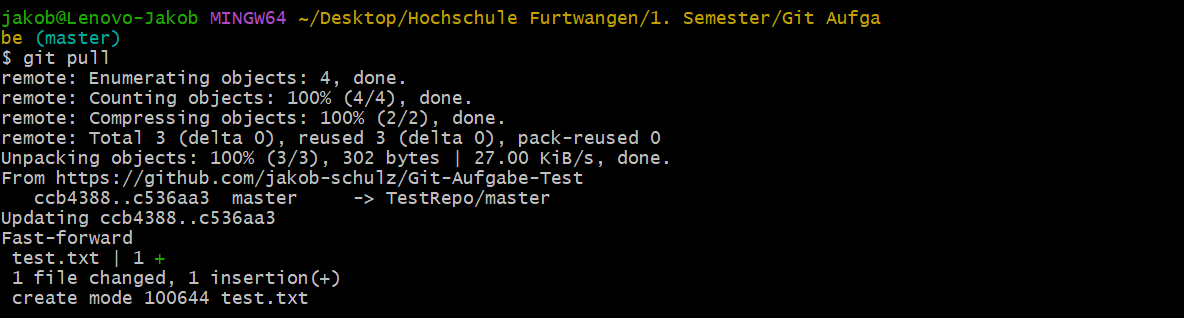
\includegraphics[width = 13 cm]{git_merge.png}\\
\\
Das funktoniert nur dann, wenn die "Anderungen an verschiedenen Stellen der Datei vorgenmmen wurden. Ansonsten entsteht ein "`merge Konflikt"'.\\
\\
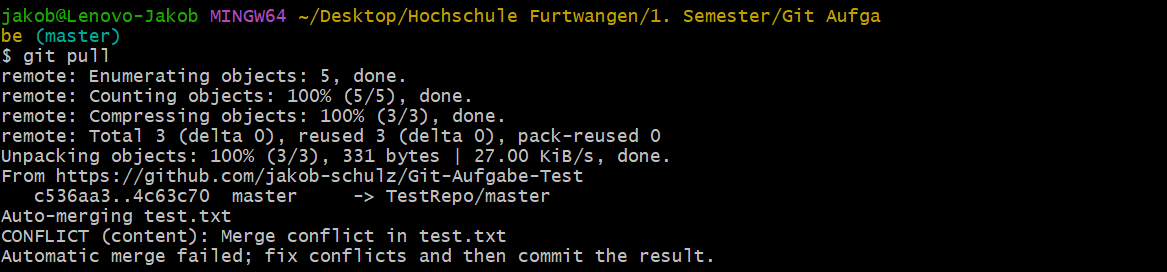
\includegraphics[width = 13 cm]{git_merge_konflikt.png}\\
\\
Nach dem merge Konflikt befindet man sich in dem Modus? master|merging. Git hat bei dem merge Konflikt die Datei im lokalen Repository und die vom online Repository in eine Datei zusammengef"uhrt. Der Anwender muss nun entscheiden, welche der "Anderungen er ben"otigt bzw. nicht ben"otigt. Damit l"ost er den Konflikt.\\
\\
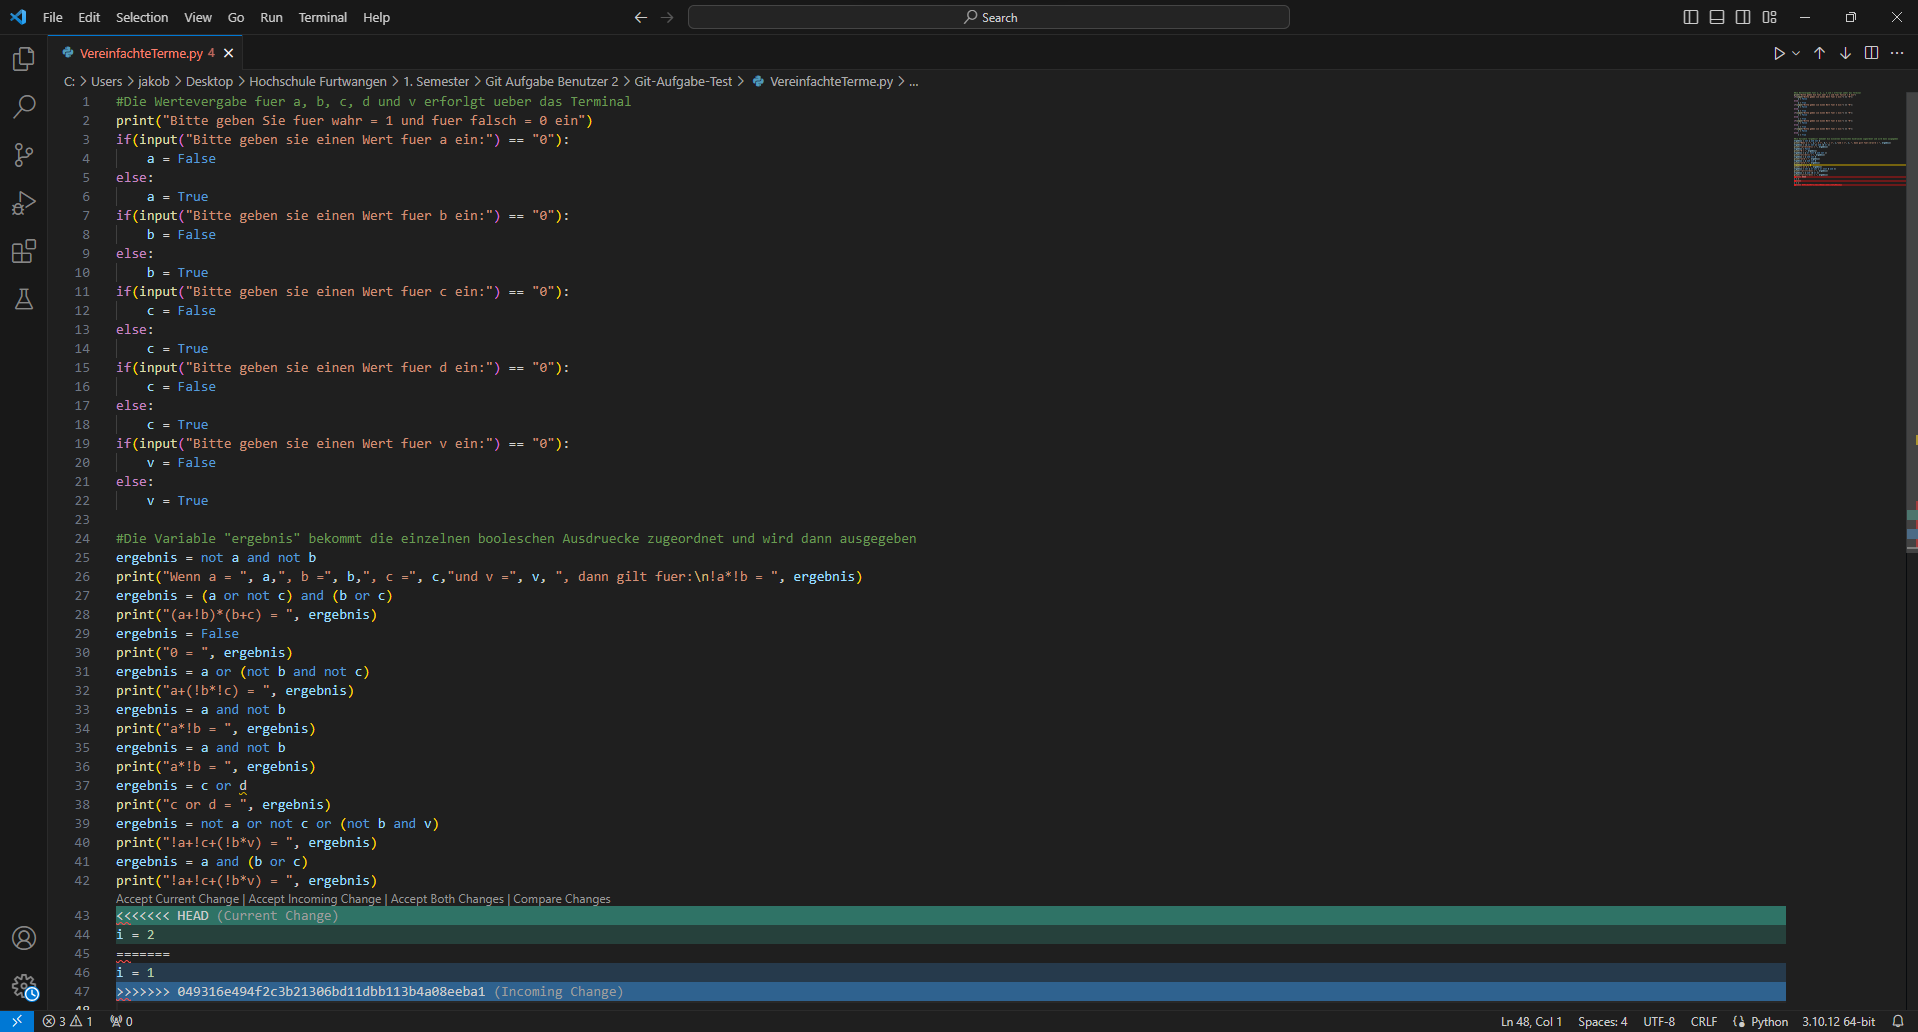
\includegraphics[width = 13 cm]{Loesen_des_Konflikts.png}\\
\\
Wichtig: Es ist nicht immer so, dass der Konflikt schoen farblich hervorgehoben wird. Dort wo es einen Konflikt gibt schreibt git einmal die Variante des online Repositorys und einmal die lokale Variante "ubereinander. Nach dem bearbeiten der Datei und l"osen des Konfliktes muss man sie wieder "`stagen"', "`commiten"' und auf das online Repository "`pushen"'.
 
\subsection{Sicherheit gegen"uber fremden Zugriff}
Zuerst einmal kann man entscheiden, ob man das Repository auf Github öffentlich oder privat machen möchte. Ist das Repository öffentlich, kann jeder es einsehen und Code davon herunterladen.\\
In den Einstellungen ("`Settings"') und dann unter "`Collaborators"' kann man bestimmte Personen hinzuf"ugen, die Zugriff auf das Repository haben d"urfen. 
Kontrollierter Zugriff kann dann durch Einladungen erfolgen.
\end{document}
